\section{Pengujian}

Tujuan pengujian adalah untuk memastikan bahwa sistem yang telah diimplementasikan memenuhi seluruh kebutuhan fungsional baik dari perspektif pengguna maupun sistem. Hasil dari pengujian ini akan memberikan gambaran terkait ketercapaian sistem dalam memenuhi kebutuhan utamanya, yaitu untuk memberikan hasil pencarian Smart Contracts yang relevan berdasarkan query dalam bahasa alami.

\subsection{Metodologi Pengujian}

Pengujian akan dilakukan dengan menggunakan sistem pencarian yang telah diimplementasikan dengan query-query yang telah disiapkan. Untuk seluruh hasil pencarian, akan dilakukan evaluasi oleh ahli domain untuk memastikan relevansi hasil pencarian terhadap query yang diberikan. Untuk setiap hasil pencarian yang relevan, akan dihitung sebagai \textit{True Positive}, sedangkan hasil pencarian yang tidak relevan akan dihitung sebagai \textit{False Positive}. Pengujian ini akan dilakukan menggunakan tiga jenis pencarian sebagai pembanding, yaitu pencarian berbasis semantik, pencarian berbasis teks pada \textit{source code}, dan pencarian berbasis teks pada deskripsi semantik. Setiap ukuran keberhasilan dapat diukur dengan metode berikut:

\begin{enumerate}
	\item \textbf{Relevansi Hasil Pencarian Smart Contract (UK1)}: Melihat hasil pengujian dari pencarian berbasis semantik yang telah diimplementasikan.
	\item \textbf{Perbandingan Hasil dengan Sistem Pencarian Berbasis Kata Kunci (UK2)}: Melihat perbandingan hasil pencarian antara pencarian berbasis semantik dengan menggunakan deskripsi kebutuhan dan kata kunci, dengan pencarian berbasis teks pada \textit{source code} Smart Contract dan deskripsi semantik yang dihasilkan.
\end{enumerate}

Selain itu, akan dilakukan analisis terkait skalabilitas sistem, terutama dalam aspek biaya, waktu, penyimpanan, latensi, dan aspek teknis. Analisis ini akan memberikan gambaran terkait kemampuan sistem dalam menangani skala data yang lebih besar. Analisis ini akan dilakukan saat proses produksi data untuk pengujian, dimulai dari proses pengambilan data, enrichment, hingga pencarian data.

Perhitungan presisi untuk \textit{True Positive} dan \textit{False Positive} akan dilakukan menggunakan sebuah rubrik penilaian. Rubrik penilaian untuk setiap query akan dibuat berdasarkan bukti yang ada di dalam \textit{source code}. Rubrik penilaian yang digunakan dapat dilihat pada Lampiran \ref{appendix:rubrik-penilaian}. Rubrik ini berdasar pada konsep dan \textit{pattern} yang umum digunakan untuk standar-standar yang dicari, ditambah juga dengan rubrik spesifik untuk maksud dari query yang digunakan.

\subsection{Batasan Pengujian}

Berikut adalah batasan-batasan yang diterapkan dalam pengujian sistem:
\begin{enumerate}
	\item Jumlah data Smart Contracts yang digunakan dalam pengujian adalah 100 Smart Contracts yang sudah diperkaya dan sudah dilabelkan dengan benar.
	\item Jumlah \textit{node} Dgraph Zero yang digunakan dalam pengujian adalah 1 buah, dengan asumsi bahwa skalabilitas dari sistem ini bergantung pada skalabilitas underlying dari DgraphDB.
	\item Pencarian dilakukan secara sekuensial, sehingga hanya terdapat satu proses pencarian yang berjalan pada satu waktu.
	\item Jumlah query yang digunakan dalam pengujian adalah 20 query yang mencakup berbagai skenario dari sederhana hingga kompleks.
\end{enumerate}

\subsection{Data Pengujian}

Pengujian akan membutuhkan dua jenis data, yaitu data Smart Contracts yang telah diperkaya dengan deskripsi semantik dan data query yang akan digunakan untuk menguji sistem.

\subsubsection{Data Smart Contracts}

Data yang digunakan untuk pengujian adalah Smart Contracts yang telah diperkaya dengan deskripsi semantik. Data ini diambil dari Blockchain Ethereum Mainnet. Proses produksi data dilakukan dengan memanfaatkan komponen-komponen yang telah diimplementasikan, yaitu Dgraph Client, Semantic Enricher, dan Parallel Enricher, sehingga menghasilkan data yang relevan secara semantik dan dapat dijadikan dasar untuk pengujian sistem.

\subsubsection{Data Query}

Selain data Smart Contracts, pengujian juga akan menggunakan data query yang akan digunakan untuk menguji sistem. Data query ini mencakup berbagai klasifikasi kebutuhan yang disambungkan dengan data yang sudah dilabelkan dan juga berbagai kompleksitas mulai dari sederhana sampai query kompleks. Data query ini disertakan dalam Lampiran \ref{appendix:query}.

\subsection{Perhitungan Metrik}

Pengujian akan dilakukan dengan menghitung metrik yang telah ditentukan sebelumnya yaitu Presisi. Metrik ini akan digunakan untuk mengukur keberhasilan sistem dalam memenuhi kebutuhan fungsional yang telah ditetapkan. Perhitungan presisi dilakukan dengan mengukur proporsi hasil pencarian yang relevan terhadap total hasil pencarian dengan rumus:

\[
	\mathrm{Presisi} = \frac{\mathrm{True\ Positives}}{\mathrm{True\ Positives} + \mathrm{False\ Positives}}
\]

\subsection{Rencana Pengujian}

Pengujian akan dilakukan menggunakan beberapa pendekatan, yaitu:

\begin{enumerate}
	\item Pengujian sistem pencarian berbasis semantik dari iterasi awal
	\item Pengujian sistem pencarian berbasis semantik dari iterasi perbaikan dengan query bahasa alami
	\item Pengujian sistem pencarian berbasis semantik dari iterasi perbaikan dengan query kata kunci 
	\item Pengujian sistem pencarian berbasis teks pada Source Code Smart Contract dengan query kata kunci
	\item Pengujian sistem pencarian berbasis teks pada deskripsi semantik dengan query kata kunci
	\item Pengujian sistem pencarian berbasis teks pada deskripsi semantik dengan query bahasa alami
\end{enumerate}

\subsection{Hasil Pengujian}

\subsubsection{Iterasi Perbaikan Sistem}
\label{subsubsec:iterasi-perbaikan-sistem}

Terdapat beberapa permasalahan yang ditemukan selama proses implementasi dan pengujian sistem ini, yang kemudian diatasi dengan melakukan iterasi perbaikan sistem. Beberapa permasalahan tersebut antara lain:

\begin{enumerate}
	\item Dgraph UID tidak \textit{stable} yang menyebabkan pengujian tidak dapat dilakukan secara konsisten untuk pelabelan data. Hal ini diatasi dengan menambahkan atribut \texttt{ContractDeployments.id} yang menggunakan atribut sebelum dilakukan \textit{enrichment} dan melakukan \textit{hashing} untuk menjadikan sebuah ID yang unik dan konsisten untuk setiap Smart Contracts. Dengan cara ini, ID tersebut akan tetap konsisten meskipun UID Dgraph berubah.
	\item Proses enrichment yang dilakukan pada data sangat bergantung pada prompt yang diberikan. Hal ini menyebabkan hasil enrichment yang dapat bervariasi. Hal ini diatasi dengan melakukan iterasi pada prompt yang digunakan untuk enrichment, sehingga hasil enrichment dapat lebih konsisten dan relevan dengan data yang ada. Iterasi ini dilakukan dengan mengubah prompt yang digunakan pada proses enrichment dan melakukan pengujian terhadap hasil yang diperoleh.
	\item Proses enrichment berdasarkan \textit{source code} Smart Contract yang dilakukan pada tahap awal tidak memberikan hasil yang optimal karena metode pemotongan yang digunakan. Secara spesifik, source code dari sebuah Smart Contract seringkali memiliki penyusunan urutan yang spesifik, dimulai dari \texttt{library} yang digunakannya terlebih dahulu sehingga mengaburkan konteks keseluruhan jika kontrak tersebut menggunakan banyak \textit{library}. Hal ini diatasi dengan menghilangkan pemotongan token. Dengan cara ini, walau biaya token meningkat, proses enrichment dapat dilakukan dengan lebih baik dan hasil yang diperoleh lebih relevan dengan data yang ada.
	\item Proses enrichment dan retrieval sangat bergantung pada format yang digunakan untuk menyimpan data. Format yang digunakan harus dapat mengakomodasi pencarian semantik yang spesifik. Hal ini diatasi dengan melakukan ekstensi dan juga perubahan atribut, sehingga dapat dengan lebih spesifik mengakomodasi kebutuhan pencarian semantik.
	\item Proses konversi menjadi embeddings membutuhkan konteks penjelasan tambahan terkait istilah-istilah spesifik domain yang digunakan. Hal ini diatasi dengan menambahkan sebuah \textit{dictionary} yang berisi istilah-istilah spesifik domain yang digunakan pada proses enrichment. Dengan cara ini, proses konversi menjadi embeddings dapat dilakukan dengan lebih baik dan hasil yang diperoleh lebih relevan dengan data yang ada. Hasil dari \textit{dictionary} ini dapat dilihat pada Lampiran \ref{appendix:embeddings-dictionary}.
	\item Pengujian membutuhkan fitur tambahan untuk melakukan \textit{benchmarking} terhadap hasil yang didapatkan. Hal ini diatasi dengan menambahkan fitur tambahan pada sistem, terutama pada bagian Dgraph Client, API, dan Web GUI untuk melakukan pencarian berbasis teks kepada \textit{source code} dan juga hasil deskripsi semantik yang dihasilkan. Dengan fitur ini, pengujian \textit{benchmark} dapat dilakukan dengan lebih mudah. Hasil perubahan ini dapat dilihat pada setiap lampiran implementasi.
	      % Bisa kasih lampiran, terus juga bilang kalau ini ada tradeoff di token, jadi lebih mahal tapi lebih baik
	      % tapi gemini disini dipake karena lebih murah dan lebih besar context windownya
\end{enumerate}

\subsubsection{Pengujian Sistem Pencarian Berbasis Semantik dari Iterasi Awal}

Hasil dari pengujian ini dapat dilihat pada Gambar \ref{image:pengujian-1}. Hasil dari pengujian ini menunjukkan rata-rata presisi sebesar 55\%. Tetapi, terdapat inkonsistensi dari hasil yang diperoleh untuk beberapa query yang diberikan, dimana terdapat query memberikan hasil yang sepenuhnya relevan, tetapi terdapat juga query yang tidak memberikan hasil yang relevan sama sekali. Hal ini menunjukkan bahwa sistem masih perlu diperbaiki, terutama dalam hasil enrichment yang dibaca oleh ahli, dimana deskripsi yang dihasilkan dinilai masih cukup umum, sehingga tidak memberikan hasil yang cukup spesifik.

\begin{table}[ht]
	\centering
	\caption{Hasil Pengujian Sistem Pencarian Berbasis Semantik dari Iterasi Awal}
	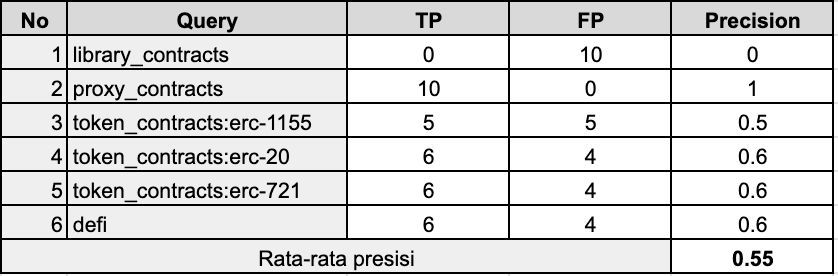
\includegraphics[width=1\textwidth]{resources/chapter-4/data-1-1.png}
	\label{image:pengujian-1}
\end{table}

\subsubsection{Pengujian Sistem Pencarian Berbasis Semantik dari Iterasi Perbaikan dengan Query Bahasa Alami}

Hasil dari pengujian ini dapat dilihat pada Gambar \ref{image:pengujian-2}. Hasil dari pengujian ini menunjukkan rata-rata presisi sebesar 65\%, peningkatan 10\% jika dibandingkan dengan iterasi awal. Hal ini menunjukkan bahwa presisi sistem dipengaruhi oleh mekanisme enrichment yang dilakukan. Selain itu, sistem dapat mendapatkan hasil spesifik dari sebuah kontrak hanya dengan mendeskripsikan isi fungsionalitas atau tujuan dari Smart Contract tersebut. Secara umum, hasil pencarian semantik yang didapatkan cukup konsisten, dimana terdapat hasil-hasil yang relevan untuk setiap query yang diberikan.

\begin{table}[ht]
	\centering
	\caption{Hasil Pengujian Sistem Pencarian Berbasis Semantik dari Iterasi Perbaikan dengan Query Bahasa Alami}
	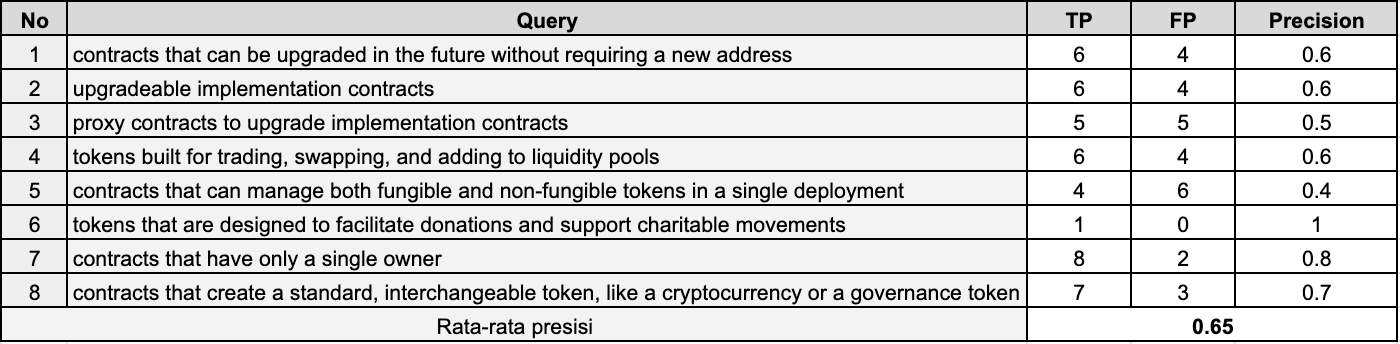
\includegraphics[width=1\textwidth]{resources/chapter-4/data-1-2.png}
	\label{image:pengujian-2}
\end{table}

\subsubsection{Pengujian Sistem Pencarian Berbasis Semantik dari Iterasi Perbaikan dengan Query Kata Kunci}

Hasil dari pengujian ini dapat dilihat pada Gambar \ref{image:pengujian-3}. Pengujian ini dilakukan dengan menggunakan query berupa kata kunci yang relevan dengan Smart Contract yang ada. Hasil dari pengujian ini menunjukkan rata-rata presisi sebesar 72,5\%, 7,5\% lebih baik dibandingkan dengan menggunakan query bahasa alami.

\begin{table}[ht]
	\centering
	\caption{Hasil Pengujian Sistem Pencarian Berbasis Semantik dari Iterasi Perbaikan dengan Query Kata Kunci}
	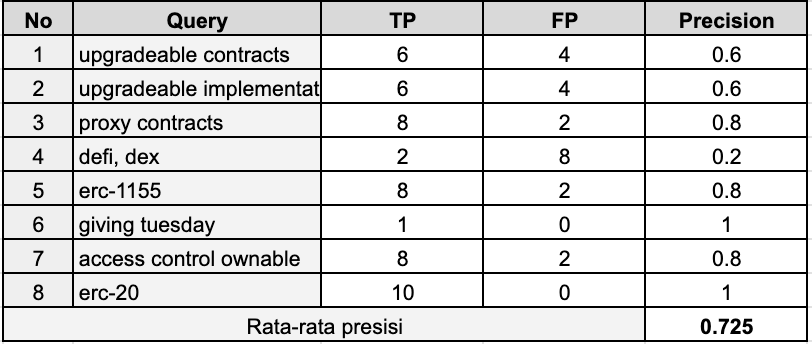
\includegraphics[width=1\textwidth]{resources/chapter-4/data-1-3.png}
	\label{image:pengujian-3}
\end{table}

\subsubsection{Pengujian Sistem Pencarian Berbasis Teks pada \textit{source code} Smart Contract dengan Query Kata Kunci}

Hasil dari pengujian ini dapat dilihat pada Gambar \ref{image:pengujian-4}. Pengujian ini dilakukan dengan menggunakan query berupa kata kunci yang relevan dengan \textit{source code} Smart Contract yang ada. Hasil dari pengujian ini menunjukkan rata-rata presisi sebesar 39\%. Faktor utama dari hasil ini adalah karena sistem hanya melakukan pencarian berbasis sintaks pada \textit{source code} Smart Contract, sehingga tidak dapat memberikan hasil yang relevan dengan konteks yang ada.

\begin{table}[ht]
	\centering
	\caption{Hasil Pengujian Sistem Pencarian Berbasis Kata Kunci pada \textit{source code} Smart Contract dengan Query Kata Kunci}
	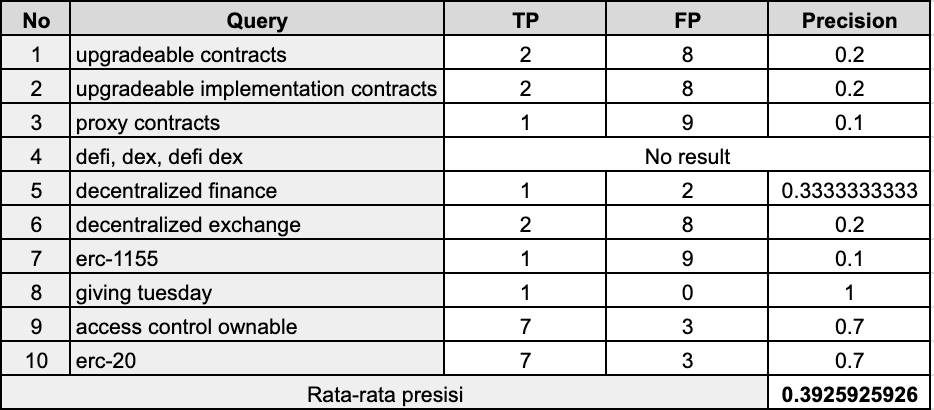
\includegraphics[width=1\textwidth]{resources/chapter-4/data-1-4.png}
	\label{image:pengujian-4}
\end{table}

\subsubsection{Pengujian Sistem Pencarian Berbasis Teks pada Deskripsi Semantik dengan Query Kata Kunci}

Hasil dari pengujian ini dapat dilihat pada Gambar \ref{image:pengujian-5}. Pengujian ini dilakukan dengan menggunakan query berupa kata kunci yang relevan dengan deskripsi semantik yang dihasilkan. Hasil dari pengujian ini menunjukkan rata-rata presisi sebesar 49\%. Hasil ini menunjukkan bahwa deskripsi semantik yang dihasilkan dapat memberikan peningkatan relevansi hasil pencarian jika dibandingkan dengan pencarian yang hanya berbasis \textit{source code}.

\begin{table}[ht]
	\centering
	\caption{Hasil Pengujian Sistem Pencarian Berbasis Kata Kunci pada Deskripsi Semantik dengan Query Kata Kunci}
	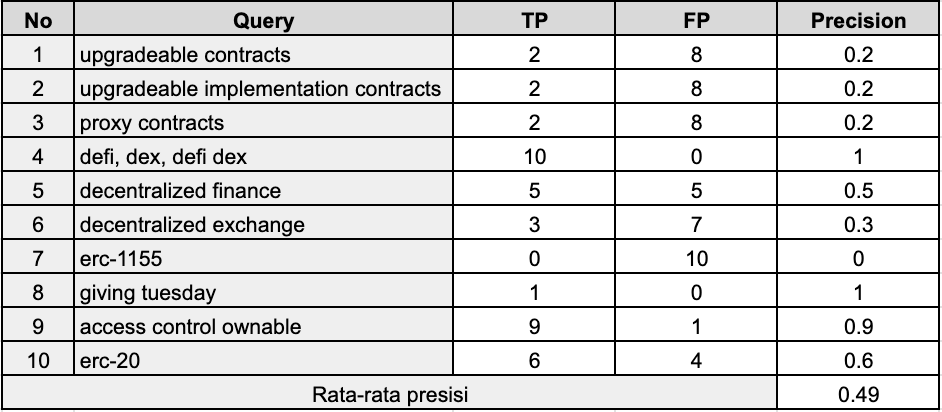
\includegraphics[width=1\textwidth]{resources/chapter-4/data-1-5.png}
	\label{image:pengujian-5}
\end{table}

\subsubsection{Pengujian Sistem Pencarian Berbasis Teks pada Deskripsi Semantik dengan Query Bahasa Alami}

Hasil dari pengujian ini dapat dilihat pada Gambar \ref{image:pengujian-6}. Pengujian ini dilakukan dengan menggunakan query berupa bahasa alami yang relevan dengan deskripsi semantik yang dihasilkan pada sistem pencarian berbasis kata kunci. Hasil dari pengujian ini menunjukkan rata-rata presisi sebesar 27,5\%. Hasil ini menunjukkan bahwa query bahasa alami tidak memberikan hasil yang relevan jika digunakan pada sistem pencarian berbasis kata kunci.

\begin{table}[ht]
	\centering
	\caption{Hasil Pengujian Sistem Pencarian Berbasis Kata Kunci pada Deskripsi Semantik dengan Query Bahasa Alami}
	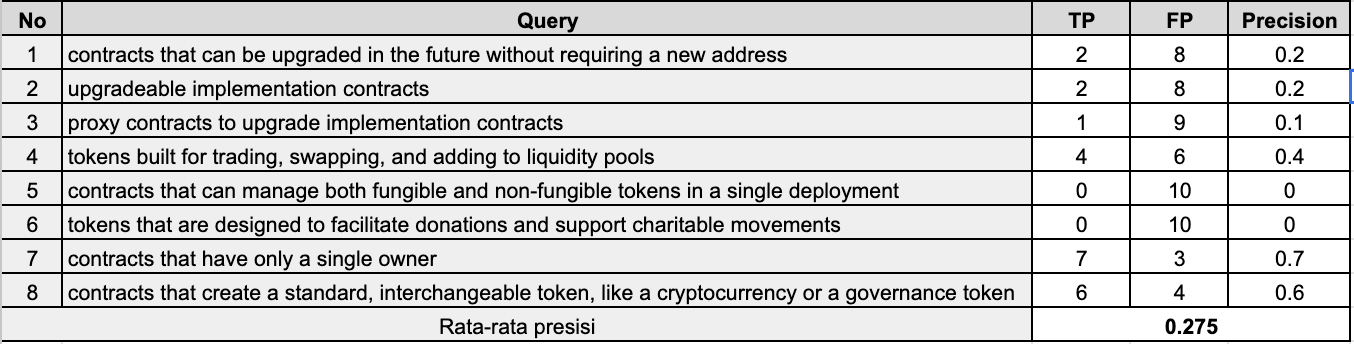
\includegraphics[width=1\textwidth]{resources/chapter-4/data-1-6.png}
	\label{image:pengujian-6}
\end{table}

\subsubsection{Teknis Sistem}
\label{subsec:teknis-sistem}

Terdapat beberapa data yang diambil dari proses enrichment untuk menilai kinerja sistem. Data ini mencakup jumlah token yang digunakan, median dari token yang digunakan, dan waktu yang dibutuhkan untuk melakukan enrichment. Tabel \ref{table:hasil-pengujian-teknis-sistem} menunjukkan hasil pengujian teknis sistem yang dilakukan pada proses enrichment. Data ini diambil dari proses enrichment yang dilakukan pada 118 Smart Contracts yang telah diperkaya dengan deskripsi semantik.

\begin{table}[ht]
	\centering
	\caption{Hasil Pengujian Teknis Sistem}
	\label{table:hasil-pengujian-teknis-sistem}
	\begin{tabular}{|l|c|}
		\hline
		\textbf{Metrik}              & \textbf{Nilai} \\ \hline
		Data                         & 118            \\ \hline
		Jumlah Token                 & 1.735.909      \\ \hline
		Biaya (GPT 4o mini)          & \$0.23         \\ \hline
		Waktu Proses P50             & 5,56 detik     \\ \hline
		Waktu Proses P99             & 9,41 detik     \\ \hline
		Waktu Proses Embeddings Mean & 0,95 detik     \\ \hline
		Waktu Proses Embeddings P50  & 0,375 detik    \\ \hline
		Waktu Proses Embeddings P99  & 2,87 detik     \\ \hline
	\end{tabular}
\end{table}


\subsection{Analisis Hasil Pengujian}

\subsubsection{Analisis Hasil Pengujian Sistem}

Secara umum, hasil pengujian sistem menunjukkan bahwa sistem pencarian berbasis semantik memberikan hasil yang lebih relevan dibandingkan dengan sistem pencarian berbasis teks. Selain itu, sistem pencarian berbasis semantik juga dapat menghasilkan relevansi yang baik untuk masukan berupa query bahasa alami dan kata kunci. Sedangkan sistem pencarian berbasis teks hanya dapat menerima masukan berupa kata kunci untuk mendapatkan hasil pencarian yang relevan. Hal ini menunjukkan fleksibilitas sistem pencarian berbasis semantik untuk menghasilkan hasil yang relevan berdasarkan jenis masukan yang berbeda.

Selain itu, hasil untuk sistem pencarian berbasis semantik pada iterasi perbaikan menunjukkan peningkatan presisi yang signifikan dibandingkan dengan iterasi awal. Hal ini menunjukkan bahwa proses iterasi perbaikan, yaitu perubahan prompt, format data, konteks \textit{source code} yang lengkap, dan penambahan deskripsi semantik, memberikan dampak positif yang terlihat terhadap relevansi hasil pencarian.

\subsubsection{Analisis Skalabilitas Sistem}

Skalabilitas sistem dapat dilihat dari aspek teknis sistem pada bagian \ref{subsec:teknis-sistem}. Untuk menilai skalabilitas sistem, diperlukan referensi jumlah data yang ada pada blockchain saat ini. Berdasarkan data dari Etherscan yang diambil pada 31 Juli 2025, jumlah Smart Contracts yang ada pada blockchain Ethereum pada network mainnet adalah 79.598.826 Smart Contracts dengan 790.354 diantaranya adalah Verified Smart Contracts. Data lengkap terkait jumlah data Smart Contracts dapat dilihat pada Gambar \ref{image:etherscan-smart-contracts}. Fokus dari sistem ini adalah pada Verified Smart Contracts, karena fokus sistem ini adalah untuk memberikan hasil pencarian yang dapat dimanfaatkan untuk digunakan ulang. Smart Contracts yang tidak terverifikasi tidak memiliki seringkali merupakan kontrak yang berbahaya, kosong, atau duplikat, sehingga tidak dianjurkan untuk digunakan ulang.

\begin{figure}[ht]
	\centering
	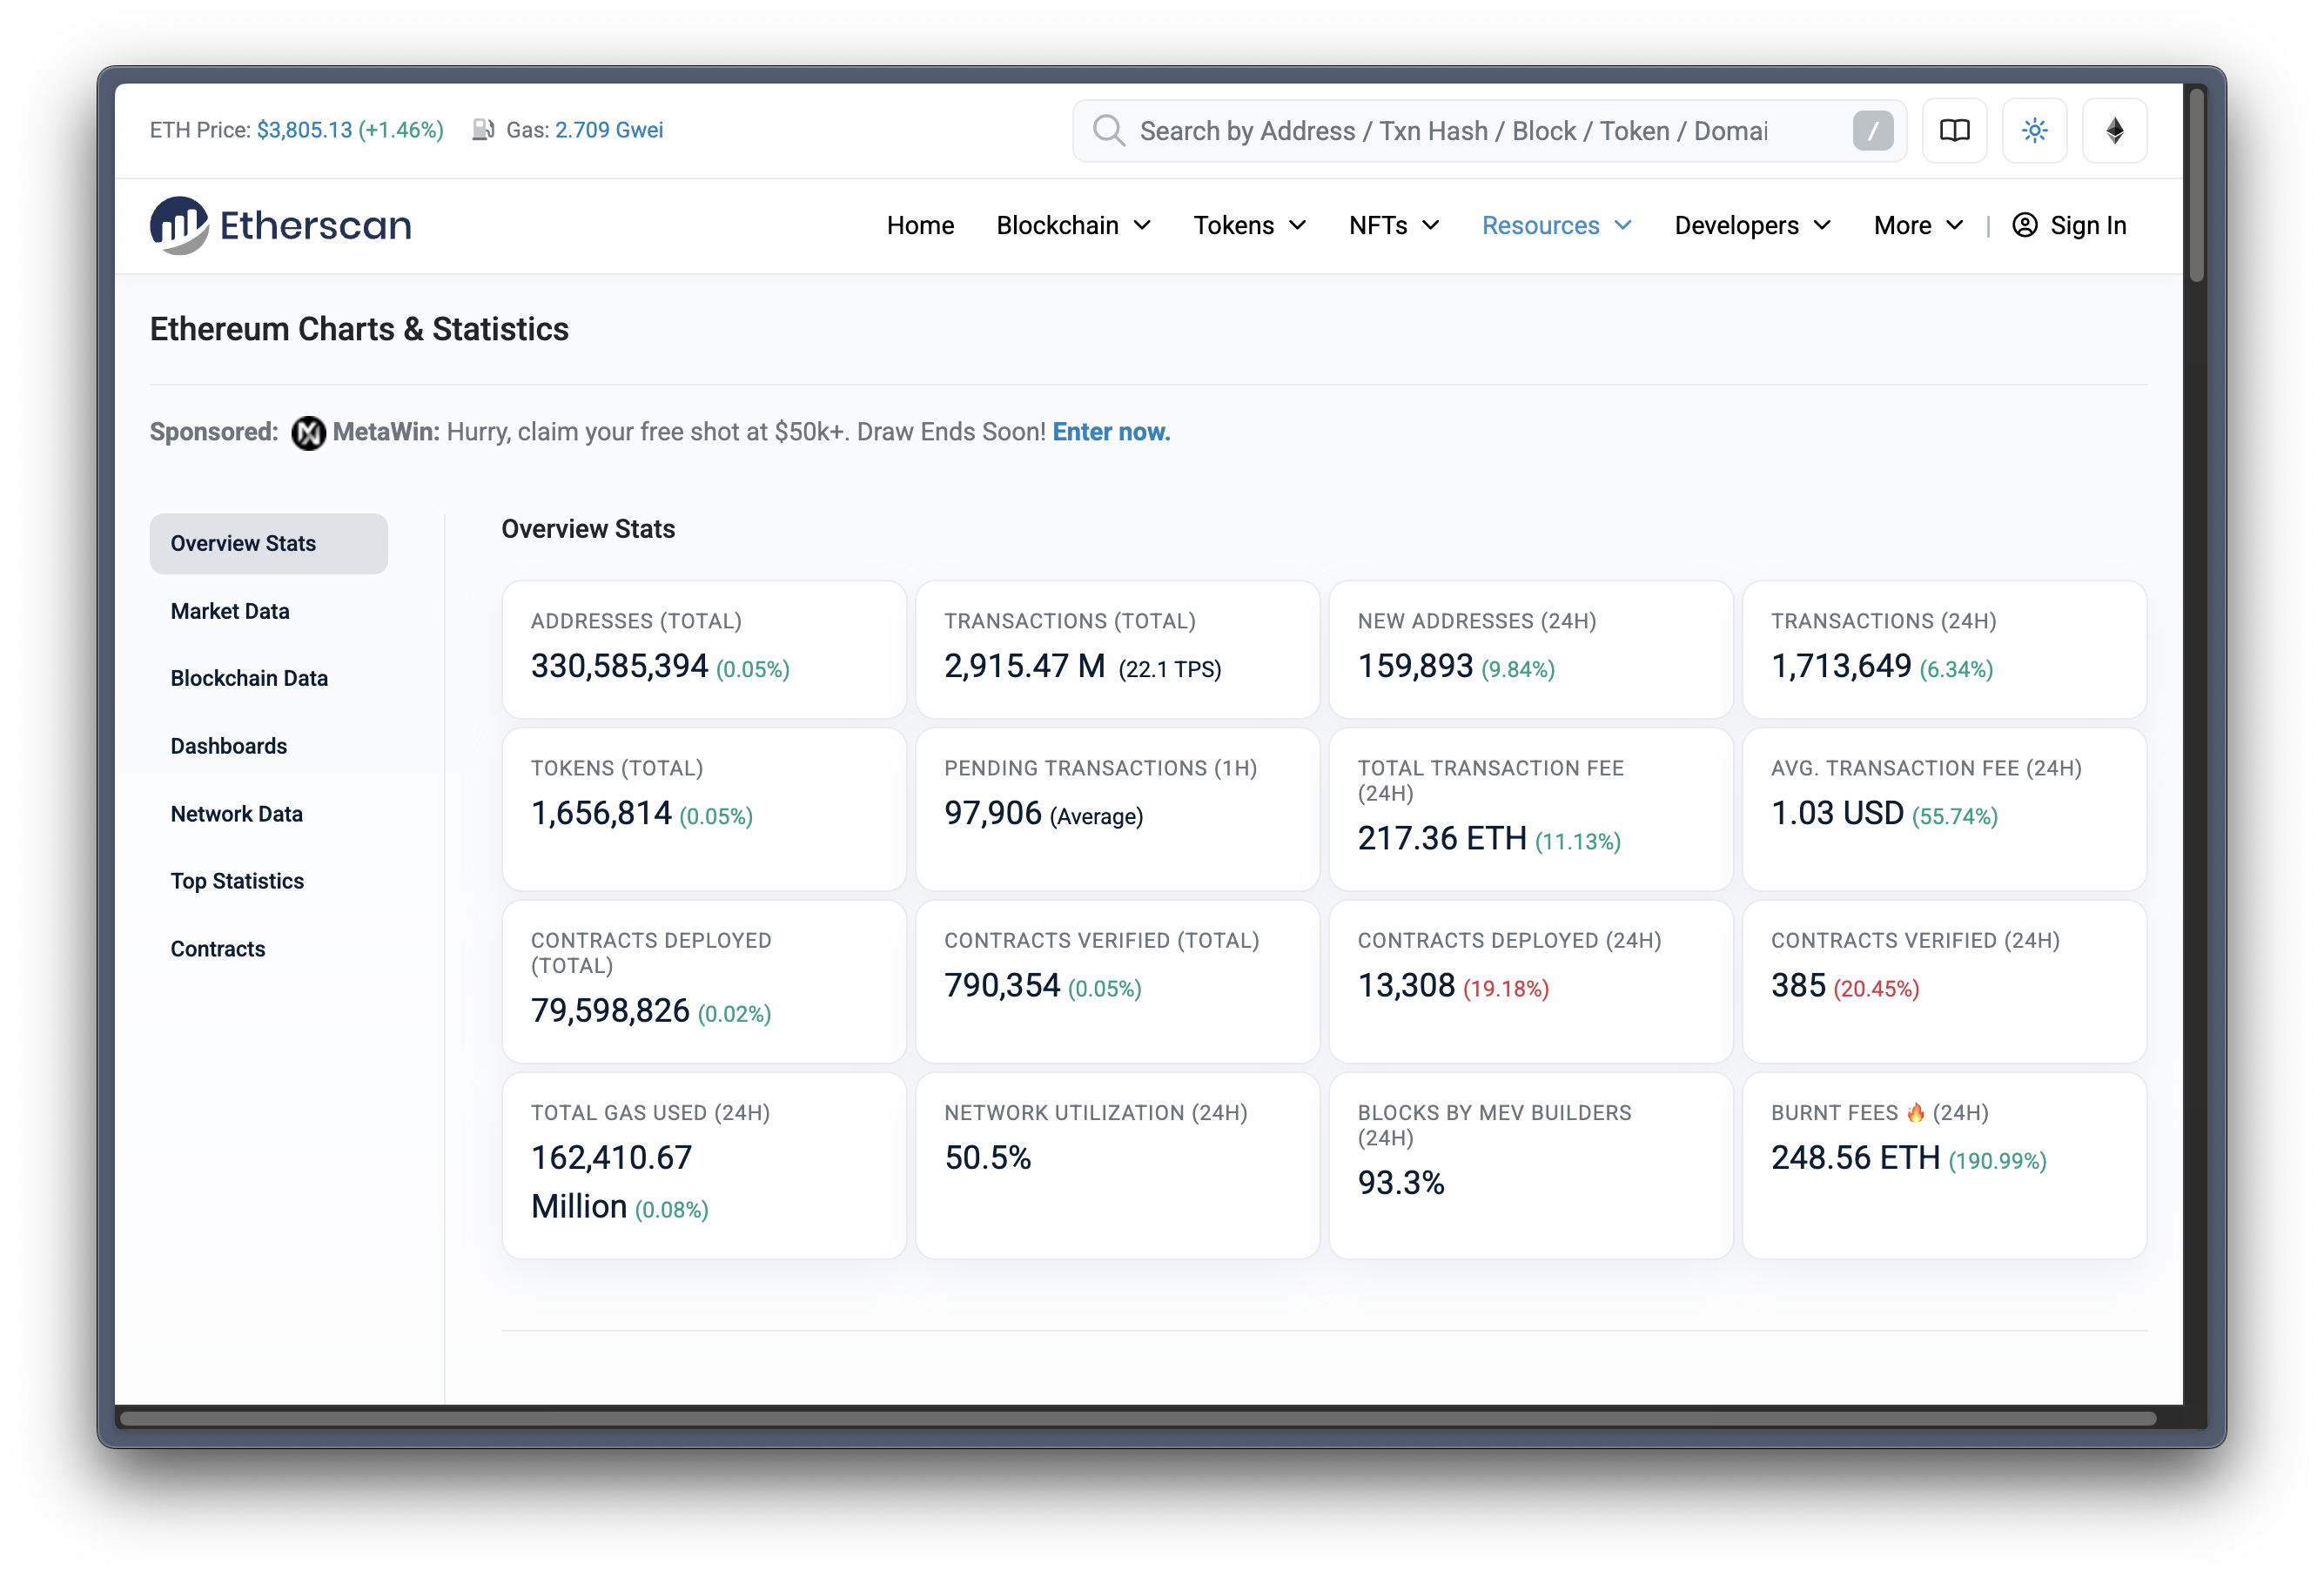
\includegraphics[width=1\textwidth]{resources/chapter-4/smart-contracts.png}
	\caption{Statistik Ethereum Mainnet}
	\label{image:etherscan-smart-contracts}
\end{figure}

Berdasarkan data yang didapatkan saat melakukan proses enrichment, didapatkan \textit{baseline calculation}:

\begin{align*}
    \text{Biaya per Kontrak} &= \frac{\text{Total Biaya}}{\text{Kontrak Diproses}} \\
    &= \frac{C_{\text{total}}}{N} \\
    &= \frac{\$0,23}{118} \\
    &\approx \$0,00195 \text{ per contract}
\end{align*}

Waktu rata-rata yang per kontrak dapat diaproksimasi menggunakan P50:
\[
\text{Waktu rata-rata per Kontrak} \approx T_{\text{P50}} = 5,56 \text{ detik}
\]

Menggunakan kedua unit tersebut, dapat ditinjau dua analisis utama, yaitu analisis skalabilitas berdasarkan biaya dan waktu.

\subsubsubsection{Analisis Skalabilitas Biaya}

Analisis akan menggunakan dua lingkup, yaitu lingkup Verified Smart Contracts, yang akan lebih mungkin untuk digunakan ulang dan semua Smart Contracts. Berikut merupakan perhitungan yang digunakan:

\begin{align*}
	C_{\text{estimated, verified}} &= N_{\text{verified}} \times C_{\text{unit}} \\
	&= 790.354 \text{ contracts} \times \$0,00195/\text{contract} \\
	&\approx \$1.541
\end{align*}

Biaya yang akan dikeluarkan untuk menganalisis seluruh Verified Smart Contracts sekitar \$1.500. Biaya ini dapat diterima secara skalabilitas karena hanya perlu dilakukan satu kali analisis dan hasil akan disimpan secara persisten sehingga tidak perlu melakukan analisis pada kontrak yang sama berulang kali.

Selanjutnya, untuk perhitungan dari biaya semua Smart Contracts:

\begin{align*}
	C_{\text{estimated, total}} &= N_{\text{total}} \times C_{\text{unit}} \\
	&= 79.598.826 \text{ contracts} \times \$0,00195/\text{contract} \\
	&\approx \$155.218
\end{align*}

Dibutuhkan biaya sebesar sekitar \$150.000 untuk menganalisis seluruh Smart Contracts yang ada pada blockchain. Hal ini menunjukkan bahwa percobaan memproses seluruh data Smart Contracts pada blockchain, termasuk jutaan kontrak kosong, simpel, atau duplikat, akan menjadi sangat mahal.

\subsubsubsection{Analisis Skalabilitas Waktu}

Waktu yang dibutuhkan akan bergantung pada kapabilitas sistem untuk memproses data secara paralel. Untuk kepentingan analisis, akan dihitung dua skenario, yaitu sekuensial atau tidak paralel, dan paralel dengan 100 proses. Berikut merupakan perhitungan yang digunakan:

\begin{align*}
	T_{\text{sequential, total}} &= N_{\text{total}} \times T_{\text{avg}} \\
	&= 79.598.826 \text{ contracts} \times 5,56 \text{ \text{s}/\text{contract}} \\
	&= 442.569.471,56 \text{s} \\
	T_{\text{sequential, verified}} &= N_{\text{verified}} \times T_{\text{avg}} \\
	&= 790.354 \text{ contracts} \times 5,56 \text{ \text{s}/\text{contract}} \\
	&= 4.394.368,24 \text{s}
\end{align*}

Waktu yang dibutuhkan untuk memproses seluruh kontrak adalah sekitar 14 tahun dan untuk seluruh Verified Smart Contracts adalah sekitar 51 hari. Hal ini menunjukkan bahwa pemrosesan sekuensial akan tidak \textit{scalable}. Tetapi, pemrosesan satu data dengan data yang lain merupakan proses yang \textit{mutually exclusive}, sehingga dapat diproses secara paralel dengan tidak terbatas. Secara teori, skalabilitas waktu dari sistem dapat terjaga dengan baik. Berikut merupakan perhitungan untuk pemrosesan paralel dengan 100 proses:

\begin{align*}
    T_{\text{parallel, total}} &= \frac{T_{\text{sequential, total}}}{P} \\
    &= \frac{14 \text{ hari}}{100 \text{ proses}} \\
	&\approx 51 \text{ hari} \\
    T_{\text{parallel, verified}} &= \frac{T_{\text{sequential, verified}}}{P} \\
    &= \frac{51 \text{ hari}}{100 \text{ proses}} \\
	&\approx 12,2 \text{ jam}
\end{align*}

Perhitungan berikut menunjukkan bahwa dengan pemrosesan paralel, waktu yang dibutuhkan untuk memproses seluruh kontrak dapat dikurangi secara signifikan. Hal yang harus diperhatikan adalah P99 sistem yaitu 9,41 detik, yang bernilai hampir dua kali dari P50, sehingga dapat membuat waktu pemrosesan lebih panjang dibandingkan perkiraan yang dihitung.

\subsubsubsection{Analisis Skalabilitas Penyimpanan}

Data utama yang disimpan pada sistem ini adalah data Smart Contracts, terutama \textit{source code} dari Verified Smart Contracts. Data yang digunakan oleh sistem, yaitu sebanyak 118 data Smart Contracts, memiliki ukuran total 2,8 MB. Referensi yang dapat digunakan untuk memperkirakan ukuran data Smart Contracts jika seluruh Verified Smart Contracts diproses adalah data dari Smart Contract Sanctuary Ethereum. Repositori ini berisikan 344.250 Smart Contracts dengan ukuran total 28 GB. Sehingga perkiraan ukuran data Smart Contracts jika seluruh Verified Smart Contracts diproses adalah sekitar 60 GB. Hal ini menunjukkan bahwa masih memungkinkan untuk sistem dapat mengakomodasi penyimpanan seluruh data Verified Smart Contracts.

\subsubsubsection{Analisis Latensi Pencarian}

Latensi pencarian pada sistem ini dapat dibagi menjadi dua, yaitu latensi pencarian pada Dgraph dan waktu pemrosesan Natural Language Query menjadi embeddings. Data latensi pencarian pada Dgraph dapat dilihat pada Gambar \ref{image:latency-dgraph}. Latensi pencarian pada Dgraph memiliki P99 sebesar 134,51 ms dan P50 sebesar 76,03 ms. Hal ini menunjukkan bahwa Dgraph dapat memberikan hasil pencarian dengan cepat. Data waktu pemrosesan Natural Language Query menjadi embeddings dapat dilihat pada Gambar \ref{image:latency-embeddings}. Waktu pemrosesan Natural Language Query menjadi embeddings memiliki P99 sebesar 2,5 detik dan P50 sebesar 73,82 ms. Hal ini menunjukkan bahwa waktu pemrosesan Natural Language Query menjadi embeddings masih dapat diterima, meskipun lebih lama dibandingkan dengan latensi pencarian pada Dgraph. Lonjakan waktu pemrosesan yang terlihat pada data disebabkan oleh lonjakan load pada CPU yang digunakan untuk menjalankan model embeddings, sehingga menyebabkan waktu pemrosesan menjadi lebih lama. Hal ini tidak akan dibahas lebih lanjut karena berada di luar lingkup topik, sehingga fokus analisis hanya pada latensi pencarian pada Dgraph.

\begin{figure}[ht]
	\centering
	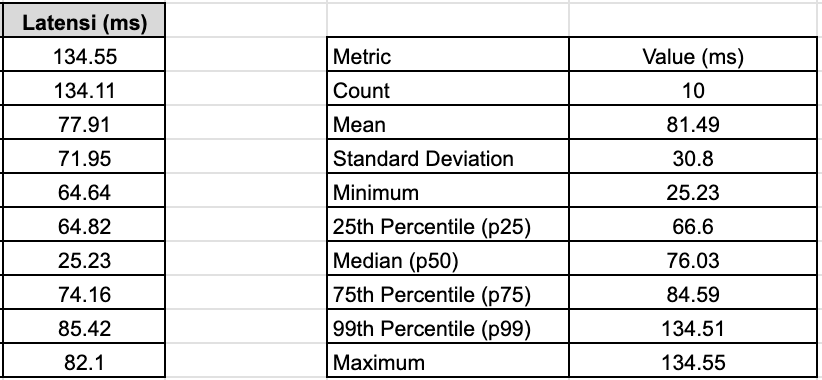
\includegraphics[width=0.75\textwidth]{resources/chapter-4/data-latensi.png}
	\caption{Statistik Latensi Pencarian pada Dgraph}
	\label{image:latency-dgraph}
\end{figure}

\begin{figure}[ht]
	\centering
	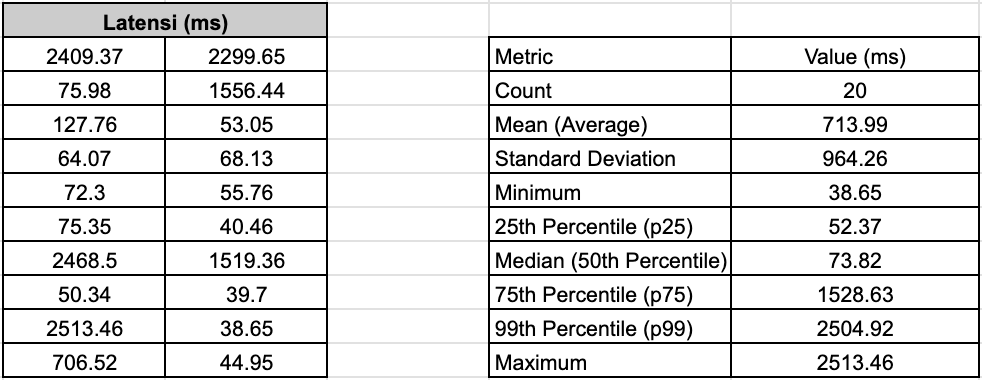
\includegraphics[width=0.75\textwidth]{resources/chapter-4/data-latensi-embeddings.png}
	\caption{Statistik Waktu Pemrosesan Natural Language Query menjadi Embeddings}
	\label{image:latency-embeddings}
\end{figure}

Secara skalabilitas, latensi pencarian pada Dgraph terbukti cukup baik saat diuji dengan 250 GB data pada pengujian yang dilakukan oleh tim pengembang Dgraph \parencite{hypermode_performance}. Dimana latensi pencarian tidak pernah melebihi 5 detik untuk seluruh pengujian yang dilakukan, bahkan untuk beban 1000 koneksi paralel dengan 2 core. Pengujian yang dilakukan oleh \cite{ashwin2016distributed} juga menjamin dari skalabilitas Dgraph. Pada lingkup Verified Smart Contracts, latensi pencarian pada Dgraph diperkirakan akan lebih baik dibandingkan dengan pengujian yang dilakukan oleh tim Hypermode, karena jumlah data yang lebih sedikit dan juga Dgraph sudah dioptimasi untuk menangani data yang lebih besar dengan skalabilitas horizontal sistem yang tinggi dengan arsitekturnya.

\subsubsubsection{Hasil Analisis Skalabilitas}

Sistem dapat dinilai cukup \textit{scalable} secara waktu, tetapi butuh perhatian khusus pada aspek biaya. Aspek biaya ini dapat menjadi lebih \textit{scalable} seiring berjalannya waktu dengan harga token yang semakin berkurang, atau dapat menggunakan model yang lebih murah dengan \textit{tradeoff} kualitas hasil enrichment, selain itu, dapat juga menggunakan model Open Source yang \textit{self-hosted} untuk meminimalisir biaya.

Secara sistem, fokus analisis hanya pada proses enrichment karena proses retrieval sepenuhnya ditangani oleh Dgraph, dengan metrik retrieval yang sudah dilakukan \textit{benchmark}, selain itu proses \textit{data loading} juga sepenuhnya ditangani oleh eth2dgraph dengan metrik yang tertera pada risetnya.


